%%
%% This is file `sample-sigconf.tex',
%% generated with the docstrip utility.
%%
%% The original source files were:
%%
%% samples.dtx  (with options: `sigconf')
%% 
%% IMPORTANT NOTICE:
%% 
%% For the copyright see the source file.
%% 
%% Any modified versions of this file must be renamed
%% with new filenames distinct from sample-sigconf.tex.
%% 
%% For distribution of the original source see the terms
%% for copying and modification in the file samples.dtx.
%% 
%% This generated file may be distributed as long as the
%% original source files, as listed above, are part of the
%% same distribution. (The sources need not necessarily be
%% in the same archive or directory.)
%%
%% The first command in your LaTeX source must be the \documentclass command.
\documentclass[sigconf, nonacm, natbib, screen, balance=False]{acmart}

% Documentation for packages
% - ACM Article Template
%    https://www.acm.org/publications/proceedings-template
% - Pseudocode typesetting CLRS-style:
%    https://www.cs.dartmouth.edu/~thc/clrscode/clrscode3e.pdf
% - Python code typesetting
%    http://ctan.uib.no/macros/latex/contrib/listings/listings.pdf
% - AMS Math
%    http://ctan.uib.no/macros/latex/required/amsmath/amsldoc.pdf
% - Graphics
%    http://ctan.uib.no/macros/latex/required/graphics/grfguide.pdf

\usepackage{clrscode3e}  
\usepackage{listings}
\lstset{language=Python, basicstyle=\ttfamily}

% based on https://tex.stackexchange.com/questions/279240/float-for-lstlisting
\usepackage{float}
\floatstyle{ruled}
\newfloat{listing}{tbph}{lop}
\floatname{listing}{Listing}
\def\lstfloatautorefname{Listing} % needed for hyperref/auroref

\citestyle{acmauthoryear}



%% end of the preamble, start of the body of the document source.
\begin{document}

%%
%% The "title" command has an optional parameter,
%% allowing the author to define a "short title" to be used in page headers.
\title{Benchmarking Sorting Algorithms In Python}
\subtitle{INF221 Term Paper, NMBU, Autumn 2020}

\author{Jon-Mikkel Korsvik}
\email{jonkors@nmbu.no}
\affiliation{}  % separates Jane's and Joe's author block

\author{Yva Sandvik}
\email{ysandvik@nmbu.no}

%% The abstract is a short summary of the work to be presented in the
%% article.
\begin{abstract}
  In this paper, we analyse \dots 
\end{abstract}


%%
%% This command processes the author and affiliation and title
%% information and builds the first part of the formatted document.
\maketitle

\section{Introduction}\label{sec:intro}

Sorting algorithms are used to solve one of the key problems of computer science known as “The sorting problem”. This involves an input sequence of n numbers $(a_1, a_2, … , a_n)$, where the output is a permutation of the input sequence such that the numbers are ordered in an ascending order. The two main aspects to a sorting algorithm is its time complexity (speed) and its space complexity (memory usage). (Kilde: Lecture 6 ipynb, Plesser)

During this investigation we have assessed the performance of the sorting algorithms listed below, under certain assumptions regarding their time complexity. We compared their performance when sorting lists containing different types of elements, as well as their performance as the length of the lists increases. 

In the following subsections we will provide theory, pseudocode as well as details surrounding the methods used when comparing the following sorting algorithms: 

\begin{itemize}

\item Quadratic algorithms
  \begin{itemize}
  \item Insertion sort
  \item Bubble sort
  \end{itemize}
\item Sub-quadratic algorithms
  \begin{itemize}
  \item Merge sort
  \item Quick sort
  \end{itemize}
\item Combined algorithm
  \begin{itemize}
  \item Mergesort switching to insertion sort for small data
  \end{itemize}
\item Built-in sorting functions
  \begin{itemize}
  \item Python `sort()`
  \item NumPy `sort()`
  \end{itemize}
\end{itemize}

\section{Theory}\label{sec:theory}

The first two algorithms we analysed were the quadratic sorting algorithms Insertion sort and Bubble sort. These two sorting algorithms are known as quadratic sorting algorithms because their time complexity is $O(n^2)$.
 
We then moved onto the sub-quadratic algorithms Merge sort and Quick sort, sharing an avreage time complexity of $O(n\lg n)$. 

Finally we compared the built in sorting algorithms Python sort and Numpy sort. 

\subsection{Algorithm 1 - Insertion sort}\label{sec:algo1}

\begin{listing}
  % Pseudocode caption above the code.
  \caption{Insertion sort algorithm from \citet[Ch.~2.1]{CLRS_2009}.}
  \label{lst:insertion_algo}

  \begin{codebox}
    \Procname{$\proc{Insertion\_Sort}(A)$}
    \li \For $j \gets 2$ \To $\attrib{A}{length}$
    \li \Do
    $\id{key} \gets A[j]$
    \li     $i \gets j-1$
    \li      \While $i>0$ and $A[i] > \id{key}$
    \li      \Do
    $A[i+1] \gets A[i]$
    \li         $i \gets i-1$
    \End    
    \li       $A[i+1]\gets \id{key}$
    \End
  \end{codebox}
\end{listing}

Insertion sort is a simple in place and comparison based sorting algorithm. Best case runtime for this algorithm is:

\begin{equation}
  T(n) = \Theta(n) \;.  \label{eq:ins_sort_best}
\end{equation}

This is achieved when the input array is already sorted. The worst case runtime occurs if the input list is in reversed order. This gives a quadratic runtime of:

\begin{equation}
  T(n) = \Theta(n^2) \;  \label{eq:ins_sort_best}
\end{equation}

The average runtime is also quadratic, making insertion sort a bad choice for sorting large lists, however it is one of the best and quickest alternatives when it comes to sorting smaller lists. 

Pseudocode for the insertion sort algorithm is shown in
listing ~\ref{lst:insertion_algo}. 

\subsection{Algorithm 2 - Bubble sort}\label{sec:algo2}

Bubble sort is know as an inefficient sorting algorithm due to its simplicity. Although bubble sort and insertion sort  grow asymptotically at the same rate $\Theta(n^2)$, the difference in bubble sort and insertion sort lies in the number of comparisons. In contrast to insertion sort, bubble sort can make numerous comparisons that do not necessarily result in a swap, making it computationally less efficient.

Pseudocode for the bubble sort algorithm is shown in listing~\ref{lst:bubble_algo}. 

\begin{listing}
  % Pseudocode caption above the code.
  \caption{Bubble sort algorithm from \citet[Ch.~2.1]{CLRS_2009}.}
  \label{lst:bubble_algo}

  \begin{codebox}
    \Procname{$\proc{Bubble\_Sort}(A)$}
    \li $n \gets \attrib{A}{length}$
    \li $swapped \gets \id{False}$
    \li $rounds \gets 0$
    \li \While $swapped:$
    \li \Do
    $swapped \gets \id{False}$
    \li \For $i \gets 0 $ \To $\id{n - rounds - 1}$
    \li     \Do
    \If $A[i] > A[i+1]:$
    \li     \Do
    $A[i], A[i+1] \gets A[i+1], A[i]$
    \li $swapped \gets \id{True}$
    \End
    \End    
    \li       $rounds + 1$
    \End
  \end{codebox}
\end{listing}


\subsection{Algorithm 3 - Merge Sort}\label{sec:algo2}

Merge sort is yet another comparison-based sorting algorithm that uses the divide-and-conquer approach which involves recursively merging together two pre-sorted arrays such that the resulting array also is sorted. (kilde: CLRS s. 30, og nettside, wikipedia). Merge sort is known to be quicker when sorting larger lists. Unlike insertion sort and bubble sort it does not iterate throught the entire list several times. 

When sorting n objects, merge sort has a consistent average and worst case performance of: 

\begin{equation}
  T(n) = \Theta(n\lg n) \;  \label{eq:merge_sort_best}
\end{equation}

The implementation we have chosen of merge sort, as well as the most common implementations, do not sort in place. Which brings us to one of the drawbacks of merge sort; its memory requirement. The memory size of the input must be allocated for the sorted output to be sorted in, hence it uses more memory space than other in place sorting algorithms. (Wikipedia). 

\begin{listing}
  % Pseudocode caption above the code.
  \caption{Merge sort algorithm from \citet[Ch.~2.1]{CLRS_2009}.}
  \label{lst:merge_algo}

  \begin{codebox}
    \Procname{$\proc{Merge\_Sort}(A)$} 
    \li \If $\attrib{A}{length}$ > 1: 
    \li \Do
    $mid \gets \attrib{A}{length}$/2: 
    \li $L\_array\gets A[:mid]$
    \li $R\_array\gets A[mid:]$
    \li $mergesort(L\_array)$
    \li $mergesort(R\_array)$
    \li $L\_index\gets 0$
    \li $L\_index\gets 0$
    \li $copy\_index\gets 0$
    \li \While $L\_index < L\_array$ $and$ $R\_index < R\_array$ 
    \li \Do
    \If $L\_array[L\_index] < R\_array[R\_index]$
    \li \Do
    $L\_index + 1$
    \li \Else:
    \li $A[copy\_index] \gets R\_array[R\_index]$
    \li $R\_index + 1$
    \End
    \End
    \li \While $L\_index < \attrib{L\_array}{length}$
    \li \Do
    $A[copy\_index] \gets L\_array[L\_index]$
    \li $L\_index + 1$
    \li $copy\_index + 1$
    \End
    \li \While $R\_index < \attrib{R\_array}{length}$
    \li \Do
    $A[copy\_index] \gets R\_array[R\_index]$
    \li $R\_index + 1$
    \li $copy\_index + 1$    
    \End
  \end{codebox}
\end{listing}

Pseudocode for the merge sort algorithm is shown in listing~\ref{lst:merge_algo}. 

\subsection{Algorithm 4 - Quick sort}\label{sec:algo2}

Quick sort is an efficient in place divide-and-conquer sorting algorithm. When implemented well it can supposedly be about two or three times faster than its main competitors, such as merge sort. 

It shares the same avreage time complexity as merge sort. However the worst case time complexity of quick sort is its main disadavantage, and is $\Theta(n^2)$ due to its need of a lot of comparisons in the worst case.  

\begin{listing}
  % Pseudocode caption above the code.
  \caption{Quick sort algorithm from \citet[Ch.~2.1]{CLRS_2009}.}
  \label{lst:quick_algo}
  
  \begin{codebox}
    \Procname{$\proc{Swap}(array, a, b)$}
    \li $array[a], array[b] \gets array[b], array[a]$
    \li \Return $array$
  \end{codebox}

  \begin{codebox}
    \Procname{$\proc{Partition}(array, start, end)$}
    \li $pivotindex \gets start$
    \li $pivotvalue \gets array[end]$
    \li \For $L\_index \gets start$ \To $end$ 
    \li \Do
    \If $array[L\_index] < pvotvalue$
    \li \Do
    $swap(array, L\_index, pivotindex)$
    \li $pivotindex += 1$
    \End
    \End
    \li $swap(array, pivotindex, end)$
    \li \Return $array, pivotindex$

  \end{codebox}

  \begin{codebox}
    \Procname{$\proc{Quick\_sort}(array, start, end)$}
    \li \If $start < end$
    \li \Do
    $array, index \gets partition(array, start, end)$
    \li $array \gets quick\_sort(array, start, index-1)$
    \li $array \gets quick\_sort(array, index+1, end)$
    \li \Return array
  \end{codebox}

  \begin{codebox}
    \Procname{$\proc{Quicksort}(array)$}
    \li $array = quick\_sort(array, 0, \attrib{array}{length} - 1$

  \end{codebox}

\end{listing}

Pseudocode for the quick sort algorithm is shown in 
listing~\ref{lst:quick_algo}. 

\subsection{Algorithm 5 - Merge sort combined}\label{sec:algo2}

Merge sort can be optimized to give "Merge sort combined" by integrating insertion sort and making it a hybrid algorithm. This takes adavantage of the fact that insertion sort performs well on smaller lists. It will therefor use fewer comparisons in the worst case than both merge sort and insertion sort, potentially making it a very efficient sorting algorithm.  

\begin{listing}
  % Pseudocode caption above the code.
  \caption{Merge sort combined algorithm from \citet[Ch.~2.1]{CLRS_2009}.}
  \label{lst:mergecombined_algo}
  
 \begin{codebox}
    \Procname{$\proc{Merge\_Sort\_Combined}(A\gets list, threshold\gets11, comb\_algo: str \gets"insertion")$} 
    \li \If $\attrib{A}{length}$ > threshold
    \li \Do
    $mid \gets \attrib{A}{length}$ / 2 
    \li $L\_array\gets A[:mid]$
    \li $R\_array\gets A[mid:]$
    \li $merge\_sort\_combined(L\_array, threshold, comb\_algo)$
    \li $merge\_sort\_combined(R\_array, threshold, comb\_algo)$
    \li $L\_index\gets 0$
    \li $L\_index\gets 0$
    \li $copy\_index\gets 0$
    \li \While $L\_index < L\_array$ $and$ $R\_index < R\_array$ 
    \li \Do
    \If $L\_array[L\_index] < R\_array[R\_index]$
    \li \Do
    $L\_index + 1$
    \li \Else
    \li $A[copy\_index] \gets R\_array[R\_index]$
    \li $R\_index + 1$
    \End
    \End
    \li \While $L\_index < \attrib{L\_array}{length}$
    \li \Do
    $A[copy\_index] \gets L\_array[L\_index]$
    \li $L\_index + 1$
    \li $copy\_index + 1$
    \End
    \li \While $R\_index < \attrib{R\_array}{length}$
    \li \Do
    $A[copy\_index] \gets R\_array[R\_index]$
    \li $R\_index + 1$
    \li $copy\_index + 1$
    \End
    \li \Else:
    \li \If $comb\_algo \gets "insertion"$
    \li \Do
    $insertion_sort(A)$
    \li \Else:
    $A \gets np.sort(A)$
  \end{codebox}
\end{listing}

Pseudocode for the merge sort combined algorithm is shown in listing~\ref{lst:mergecombined_algo}. 

\subsection{Algorithm 6 - Python "sort()" }\label{sec:algo2}



\subsection{Algorithm 7 - Numpy "sort()" }\label{sec:algo2}

\section{Methods}\label{sec:methods}

Short description of what we have done so far and how:
\begin{itemize}
\item Our test data is generated using the class function ArrayGenerator found in our utility file.
\item First test data is generated, then our benchmark function times how long each algorithm uses to sort given lists with given lengths.  
\item The timer function times each test a given number of repetitions and returns all the results (so that they can be saved and used later), as well as showing the mean.
\item Mac OS and Windows 10, Python version 3.8.3 and 3.29?
\item Git hashes are provided in table 1.
\end{itemize}

\begin{listing}
  % Listing captions above the listing.   
  \caption{Expert from benchmark code.}
  \label{lst:bench_setup}
  \begin{lstlisting}
for algorithm in kwargs['function_list']:
     array_copy = copy(kwargs['array'])
     record[algorithm.__name__] = []
     for _ in range(iters):
         start_time = time.perf_counter()
         algorithm(array_copy) # Runs algo
         end_time = time.perf_counter()
   times.append(bench(func, n))
   
  \end{lstlisting}
\end{listing}

\begin{table}
  % Table captions always come *above* the table.
  \caption{Versions of files used for this report; GitLab repository
    \url{https://x.y.z}.}
  \label{tab:hashes}
  \begin{tabular}{ll}
    \hline
    File & Git hash \\\hline
    \verb!utility.py! & \verb!8ec07210f! \\
    \verb!src! & \verb!396d8a309! \\
    \verb!plot_creation.ipynb! & \verb!8ec07210f! \\
    \verb!benchmark_results.csv! & \verb!88c28d55c! \\\hline
  \end{tabular}
\end{table}

\section{Results}\label{sec:results}

\begin{figure}
  \centering
  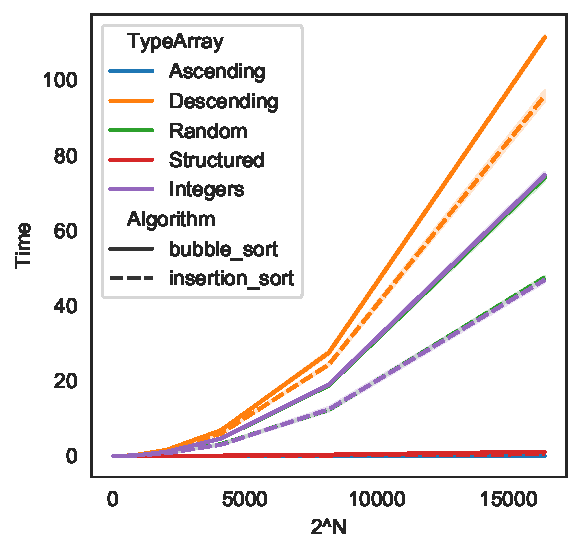
\includegraphics{foo}
  % figure captions below figure
  \caption{Benchmark results for insertion sort and bubble sort.}
  \label{fig:bench}
\end{figure}

Until now have found that insertion sort and bubble sort which are quadratic in time complexity combined with other methods like for example merge sort, drastically reduce sorting time by reducing the callstack and memory complexity. Shown in results, by optimizing the difference beneath merge sort.

\section{Discussion}\label{sec:discussion}

In this section, you should summarize your results and compare them to
expectations from theory presented in Sec.~\ref{sec:theory}.

% In the acks section, you can thank people for help.
\begin{acks}
We are grateful to \dots for \dots.
\end{acks}


%% The next two lines define the bibliography style to be used, and
%% the bibliography file.
\bibliographystyle{ACM-Reference-Format}
\bibliography{References
Iterative Quick Sort - GeeksforGeeks. 2020. GeeksforGeeks. https://www.geeksforgeeks.org/iterative-quick-sort/?fbclid=IwAR2ziWGZKt7nrgiD94kKu2if00gLmh3j2oNR6DUnSsL2b1AoLMsjvpARgYk.}
\bibliography{Insertion sort. 2020. En.wikipedia.org. https://en.wikipedia.org/wiki/Insertion_sort.}
\bibliography{Comparison of Sorting Algorithms. 2020. Medium. https://medium.com/@tssovi/comparison-of-sorting-algorithms-298fdf037c8f.}

\end{document}
